\documentclass[12pt]{article}
\usepackage[utf8]{inputenc}

\usepackage[symbol]{footmisc} % footnote symbols

\usepackage{graphicx}
\graphicspath{ {output/} } % compile mode must be normal for images to display

\usepackage[
    letterpaper, 
    portrait, 
    margin=1in]{geometry} % set paper size, orientation, and margins
    
\usepackage[
    backend=biber,
    style=apa]{biblatex} % Imports biblatex package
    
\addbibresource{ref.bib} % Import the bibliography file

% set line spacing
\setlength{\parindent}{3em}
\setlength{\parskip}{0em}
\renewcommand{\baselinestretch}{1.5}

\renewcommand{\thefootnote}{\fnsymbol{footnote}}




\begin{document}

\hspace{5pt}

\Large
 \begin{center}
High-Resolution Estimates of Agricultural Land Value for Conservation\footnote[2]{Gold and Binder acknowledge financial support from the David \& Lissa Leege Endowment and professional development grant funds from the Faculty Life Committee of St Olaf College. They would also like to thank Sara Dale and Craig Rice for their indispensable technical assistance.}\\ 
% I need to verify that I'm acknowledging the funding sources properly.
% Should we also acknowledge Rushikesh's research assistance last fall? I'm not sure what meets the acknowledgement threshold.

\vspace{10pt}

% Authors
\large
Asa Gold$^1$, Seth Binder$^1$, Christoph Nolte$^2$ \\

\vspace{10pt}

\footnotesize  
$^{1}$St. Olaf College\\ %Should I list University of Chicago, as well? Since I'm not a professor at either STO or UChicago, does it matter?
$^2$Boston University

\vspace{40pt} 

    \normalsize
    \textbf{Abstract}
\end{center}

\small
Planning for cost-effective conservation requires reliable estimates of land costs, spatially-differentiated at high resolution. Nolte (2020) provides an estimation approach that dramatically improves estimates for undeveloped land. Much undeveloped land of conservation interest is under threat of conversion to agricultural use or is already agricultural. Here we improve on the accuracy and coverage of estimation models for such land by incorporating additional variables known to affect agricultural land value and by modeling at scales corresponding to regional agricultural markets. Our estimates improve accuracy by X percent on average and extend coverage by Y percent. 

\newpage

Agencies and private organizations designing conservation efforts must contend with the fundamental scarcity of available resources, while simultaneously confronting a vast array of potential conservation strategies. Accurately predicting costs of competing strategies, then, is crucial to the cost-effective use of scarce conservation dollars. Such use, however, is often impeded the poor quality of estimates at planners' disposal concerning the fair market value of the underlying land. As recent work has demonstrated, previous efforts to predict fair market value have systematically and substantially underestimated costs of conservation (\cite{Nolte2020High-resolutionStates}). Particularly problematic has been farmland, a primary target for conservation advocates, either as a bulwark against further development or to recover natural ecosystems from degrading agricultural practices, such as monocropping. But because farmland value does not exhibit dynamics identical to those of other land types, appraisals that do not address agricultural property as a unique category might fail to accurately portray the costs of bringing farmland (or other arable land) under the aegis of regulatory agencies or non-profits like The Nature Conservancy. In Nolte's (2020) analysis, the massive scope does not treat the drivers of agricultural land value as distant from other land types.

\par Expanding Nolte (2020)'s work, we add variables on soil type, irrigation, and climatic conditions, and employ three distinct modeling strategies (linear regression, AIC ----FINALIZE----, and random forest) at three geographic levels (county, farm resource region, and national). In focusing solely on agricultural (and potentially agricultural) land, we are able to more fully capture the particular drivers of land valuation in agriculture-specific markets, contributing to more informed private and public decision making.  

BRIEF DESCRIPTION OF FINDINGS

\section{Background}
Beginning in the 1990s, environmental and land economics developed a rich literature under the broad class of Ricardian land value estimation, in which traditional econometric models are fit to data on observed sale price and climate conditions to unveil how physical features of a property are capitalized into its market value. Since (\cite{Mendelsohn1994TheAnalysis}), the Ricardian technique has been used to estimate the value of a variety of environmental factors, focusing especially on how agricultural land value and productivity respond to climatic changes (\cite{Schlenker2005WillApproach}; \cite{Schlenker2006TheConditions}; \cite{Nelson2014ClimateShocks}; \cite{Mendelsohn2003ClimateAgriculture}; \cite{Bozzola2018AAgriculture}). More recent work has produced evidence of highly nonlinear relationships between, for instance, agricultural yields--a core factor in valuation--and anthropogenic climate change (\cite{Schlenker2006NonlinearYields}; \cite{Schlenker2009NonlinearChange}), suggesting modeling approaches should move beyond mere linear panel regression techniques traditionally used in the literature.

\par Today, a more empirical approach grounded in machine learning and data science has emerged, using a diverse array of cost proxies to estimate some variation of land value nationwide (\cite{Withey2012MaximisingUSA}; 
\cite{Johnson2020AReduction}; \cite{Lawler2020PlanningConfiguration}), with Nolte (2020) marking the most recent and, to our knowledge, most accurate and validated effort. The high resolution and massive scale (N = 6.01 million) of Nolte's data, enabled in part by Zillow's limited-offer ZTRAX repository, allows for parcel-specific analysis down to fractions of a hectare (\cite{Zillow2019ZTRAX:2019-Q4}). For comparison, the USDA's National Agricultural Statistics Service land value estimates operate at a resolution of around one square mile (\cite{USDepartmentofAgriculture2019AgriculturalEstimates}). Nolte's models employ variables on location, built environment, local demographics, and physical landscape features. 

\par Informed by the literature that has demonstrated the causal effects of key environmental factors on agricultural productivity and land value, we add climatic, soil, and irrigation variables to the set of \cite{Nolte2020High-resolutionStates} predictors. Recognizing that related land markets--for example, for residential real estate--can influence the price of agricultural land, we also incorporate as predictors county-level house price indices. In addition, we test models at the scale of USDA farm resource regions to extend geographic coverage and guard against over-fitting.  

\section{Data and Methods}
We base our analysis on data first published by Nolte (2020), a comprehensive high-resolution dataset of parcel characteristics and sales across the contiguous United States (140.9 million properties across 3,055 counties), including variables on building presence, development, accessibility, local demographics, local nature preservation, terrain, water, flood risk, land cover type, location, and date of sale. To these base data, we add variables for soil quality, climate, irrigation status, and local real estate prices.

Soil classifications, indicating a map unit's suitability for agricultural use, were compiled from the Natural Resources Conservation Service (NRCS)’s high-resolution SSURGO soil survey database (\cite{SoilSurveyStaffSoilStates}). The NRCS soil survey provides map unit polygons that describe soil components (e.g., ``loamy fine sand, 0 to 2 percent slopes") and characteristics, including water capacity, flooding frequency, farmland classification, and features limiting development, among others. Soil farmland classifications indicate a map unit's suitability for agriculture fall under five general classes, defined by the USDA:
\begin{enumerate}
    \item Prime, optimal site composition and availability for producing agricultural product;  
    \item Unique, soil producing high-value crops (e.g., vineyards in California); 
    \item Statewide Importance, state-defined agricultural land that fails to meet prime criteria;
    \item Local importance, locally defined agricultural land that fails to meet prime or statewide criteria
    \item Conditional classes, land that would be considered prime, statewide importance, or local importance conditional on a specified improvement (e.g., "Prime if drained and protected from flooding")
\end{enumerate}

Farmland classifications are operationalized as the percent of each parcel containing a given classification (e.g., “Prime Farmland” or “Farmland of Statewide Importance”). Aggregation is applied to overlapping classifications containing multiple conditions. For instance, "Prime if drained or protected from flooding" gets assigned to "Prime if drained" and Prime if protected from flooding." 

30-year, monthly climate normals of minimum, mean, and maximum temperature, as well as dew temperature and precipitation come from the PRISM Climate Group (\cite{PRISMClimate2021}). We aggregate these to the meteorological season. Parcel irrigation status is based on annual 1997-2017 estimates at a resolution of 30 sq. meters, produced by the Landsat-based Irrigation Dataset, or LANID-US (\cite{Xie2021MappingStates}). We create two binary irrigation variables to record 1) whether the parcel had ever been irrigated prior to sale, and 2) whether it was irrigated at any point in the 3 years immediately preceding the sale. 

To incorporate information on local real estate markets, we add yearly all-transaction house price index values at the county level (\cite{FederalHousing2022}).

To focus our analysis on agricultural land value, we filter the ZTRAX data to only include parcels that are undeveloped, agricultural, or potentially agricultural (see Appendix for complete filtering criteria).
Our filter results in 5.26 million unique sales observations nationwide, split into testing (\textit{n = 1.47 million}) and training (\textit{n = 3.78 million}) sets stratified along the outcome variable (Fig. \ref{fig:train_test}).

\begin{figure}
    \centering
    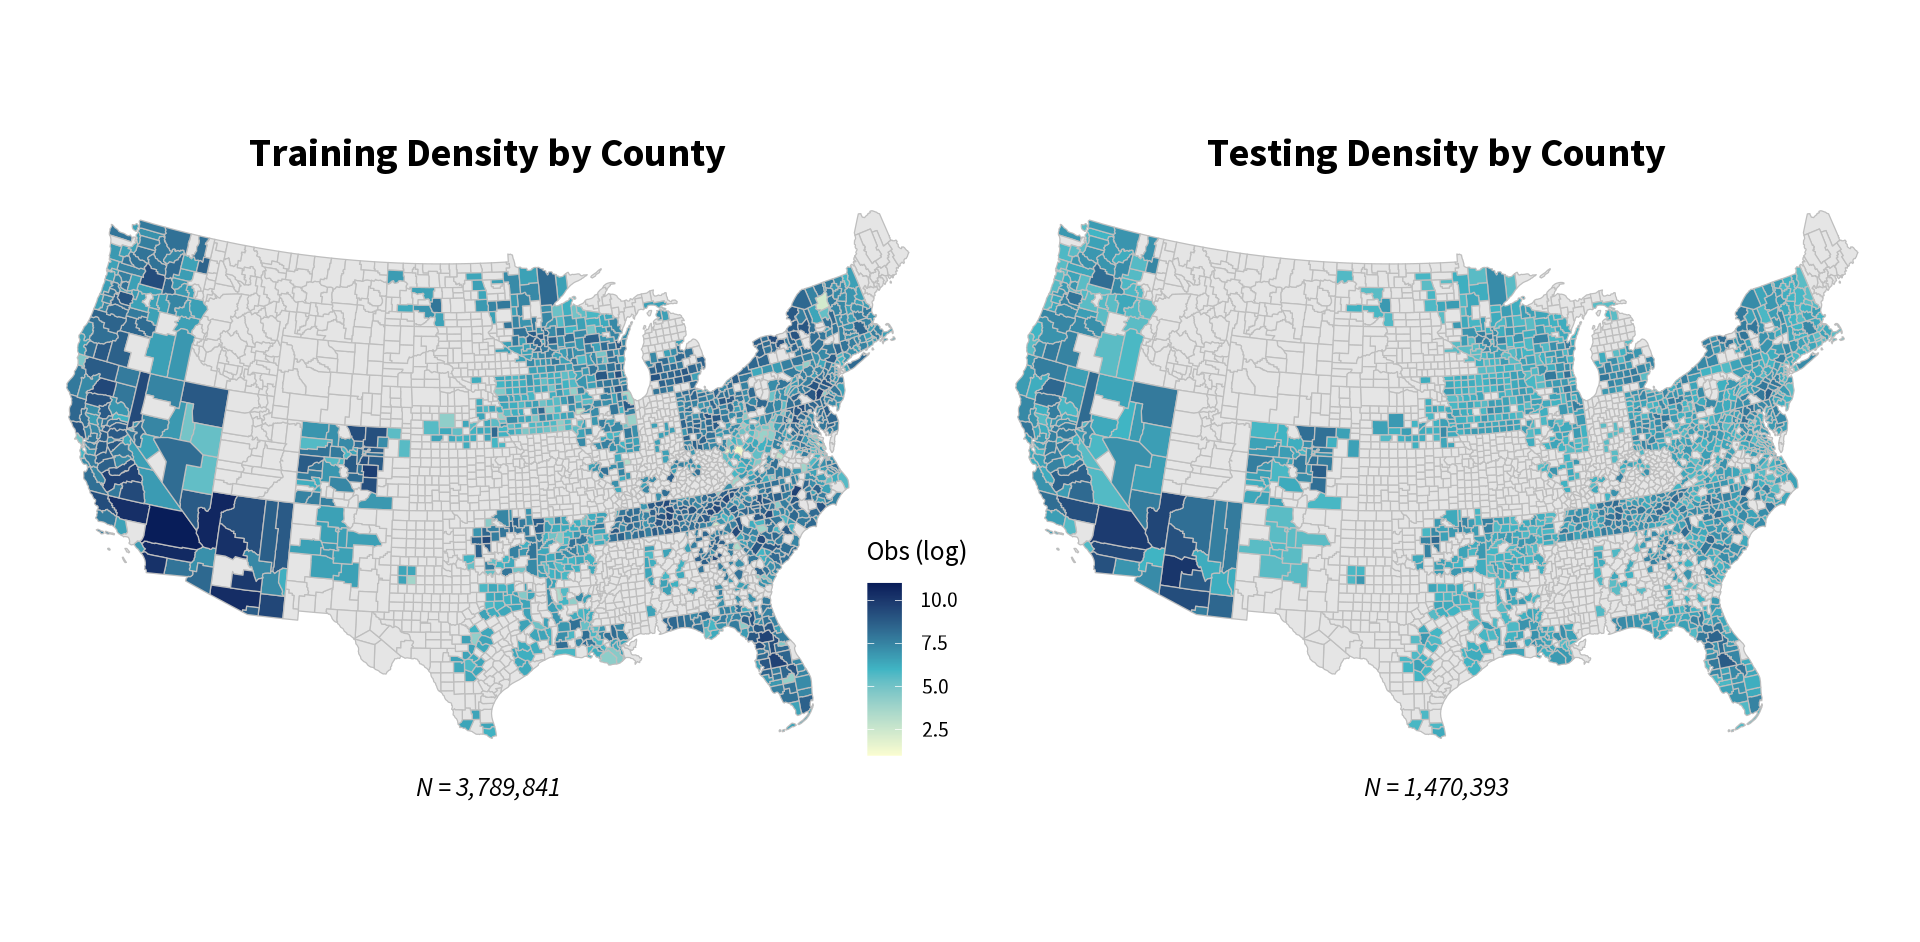
\includegraphics[width=6in]{figures/test_train_density.png}
    \caption{Observation density by training and testing sets}
    \label{fig:train_test}
\end{figure}

With this expanded dataset, we model the fair market value of parcels--measured as logged per-hectare price, adjusted for inflation using monthly consumer price index (CPI) values (\cite{blsConsumerPrice})--in two ways: linear regression and extremely randomized trees, a decision tree-based bagging algorithm. We compare these statistical approaches based on predictive accuracy, explanatory power, and variable importance or significance. Following Nolte (2020), the analysis is parallelized at the county level. Counties with fewer than 1000 observations are augmented with randomly sampled sales from adjacent counties until the focal county reaches 1000 observations. If the county and its neighbors combined fail to achieve 1000 observations, no model is specified. We specify further models at the farm resource region level. Each linear regression exists in two forms: a baseline model including all 27 variables in Nolte (2020)’s analysis, as well as our added climate, soil, and irrigation variables; and a parsimonious model selected using Akaike information criterion. Extremely randomized trees are built with 500 base learners (trees), $\frac{p}{3}$ random features tried at each split, where $p$ is the total set of predictive features, and a required minimum leaf size of 3.

\newpage

\section{Results}

RESULTS
\subsection{County-level results}
 \subsubsection{Variable importance}
 \subsubsection{Model comparison, all parcels}
 \subsubsection{Model comparison, ag parcels}
 
\subsection{Farm resource region results}
 \subsubsection{Variable importance}
 \subsubsection{Model comparison across scales, on common parcels}
 \subsubsection{Relative performance as function of observation density}
 \subsubsection{FRR model performance for additional counties}
 
 \begin{enumerate}
    \item How much extra coverage?
    \item At what accuracy?
 \end{enumerate}
 
  
\subsection{Predictive power over time}

\begin{enumerate}
    \item MSE vs time, w/ and w/o HPI, within training sample year range
    \item MSE and R2 in 2020 w/o and w/o HPI 
\end{enumerate}

 
 
\begin{figure}
    \centering
    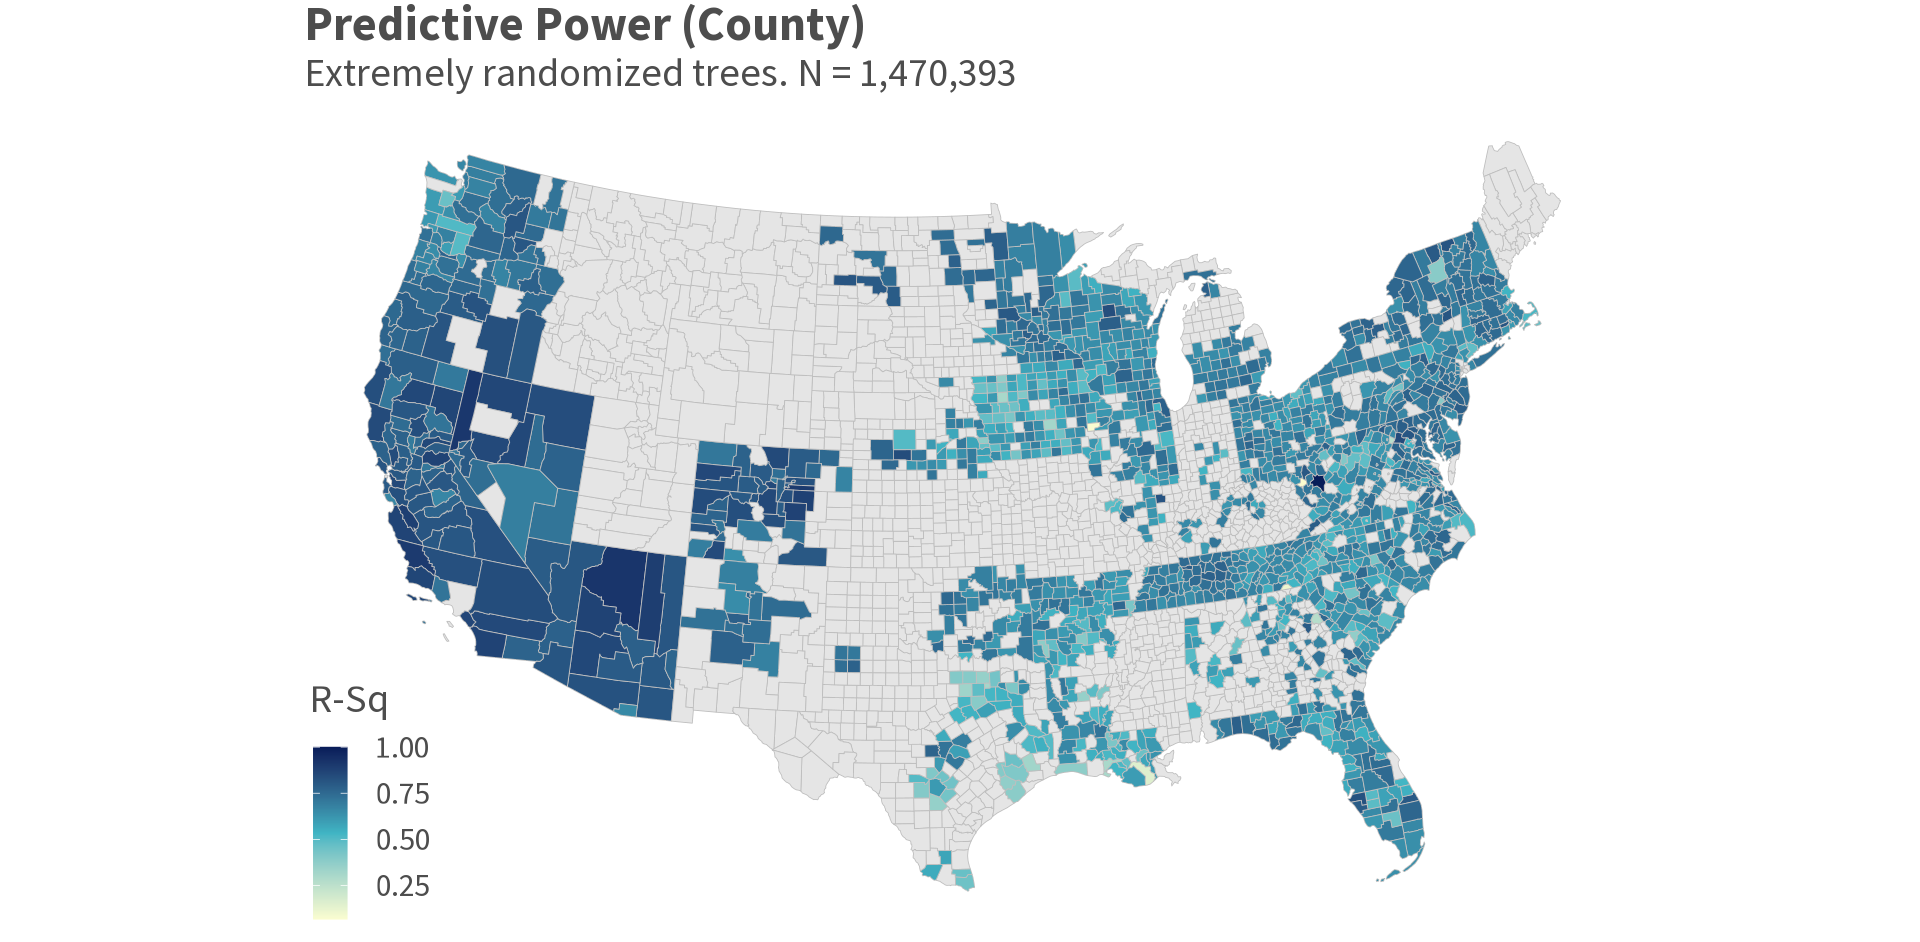
\includegraphics[width=6in]{figures/rf_rsq_map.png}
    \caption{Sales By County}
    \label{fig:rsq_county}
\end{figure}

\begin{figure}
    \centering
    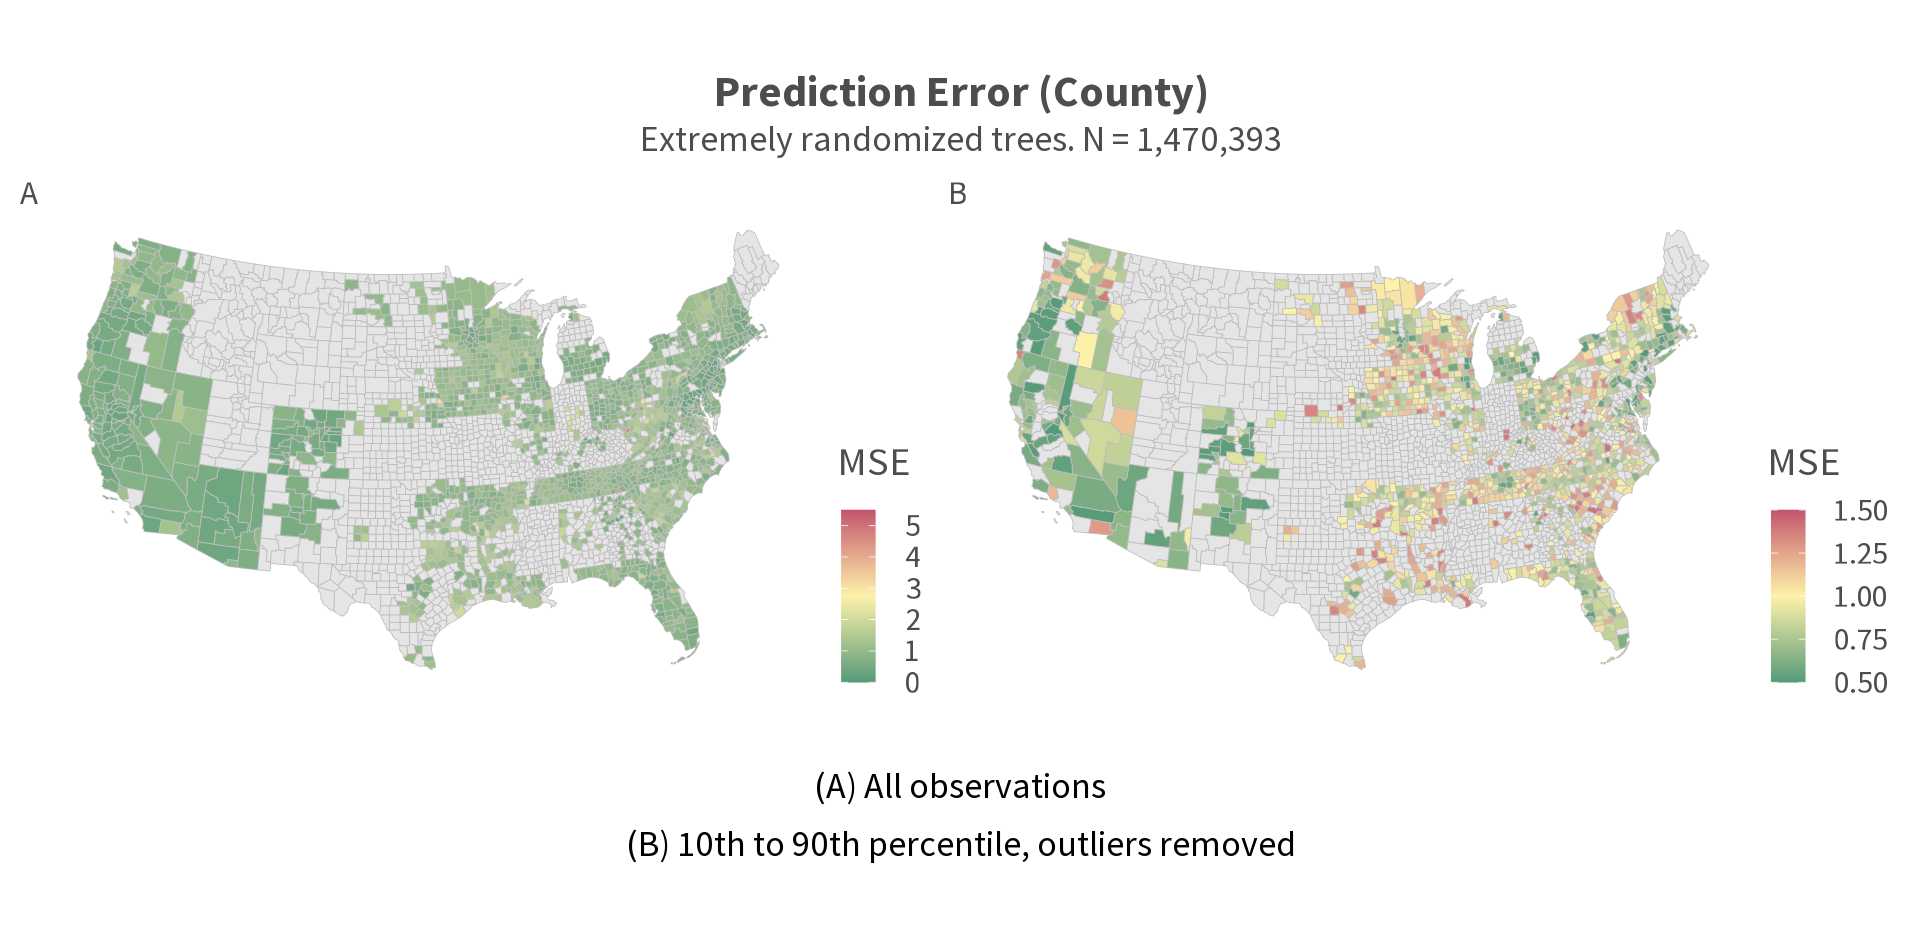
\includegraphics[width=6in]{figures/rf_mse_map.png}
    \caption{Model Performance: Prediction Error}
    \label{fig:mse_county}
\end{figure}

\newpage

\begin{figure}
    \centering
    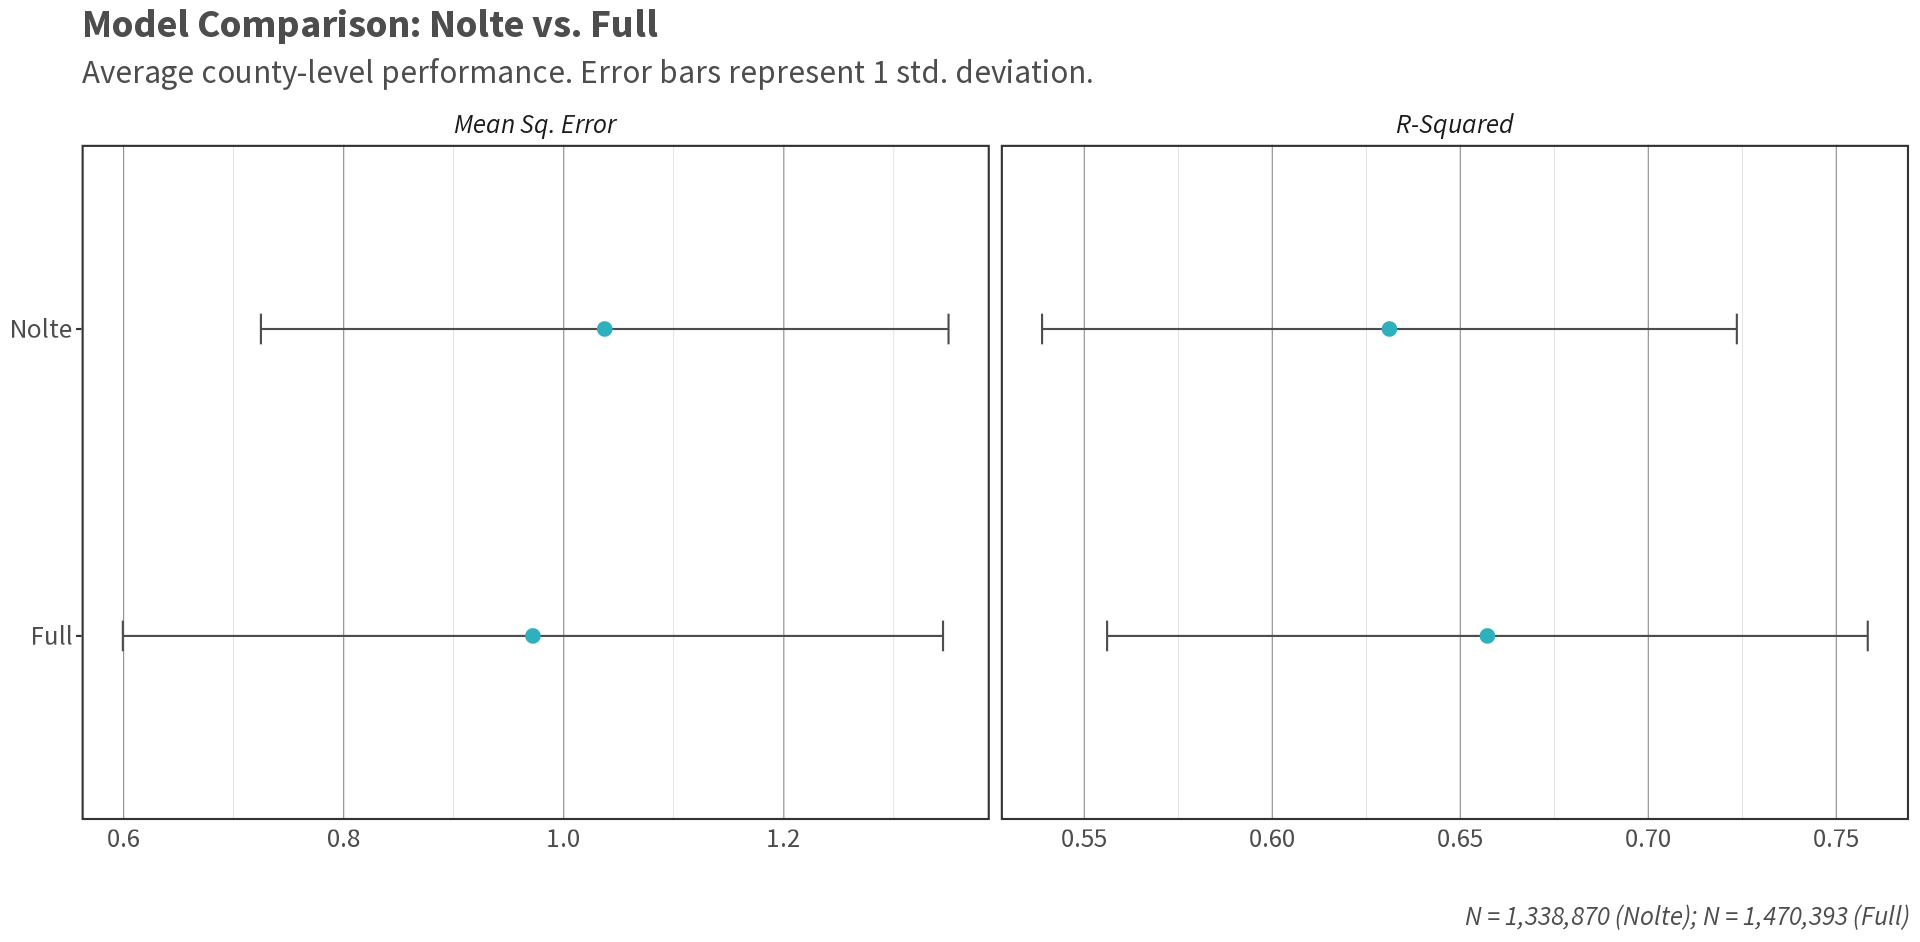
\includegraphics[width=6in]{figures/nolte_full_compare.png}
    \caption{Model performance: Only Nolte features vs. all features model}
    \label{fig:nolte_full_compare}
\end{figure}

\newpage

\section{Discussion}

DISCUSSION

\newpage

\section{Conclusion}

CONCLUSION

\newpage

\section{Appendix}


\subsection{Parcel filter}

\begin{enumerate}
    \item Meets ``undeveloped" criteria established by Nolte (2020), \textbf{or}
    \item Over half its area was classified as either grassland/herbaceous or planeted/cultivated in the 2011 National Land Cover Database (NLCD), \textbf{or}
    \item Over half its area was classified as agricultural in the 2000 Land Change Monitoring, Assessment, and Projection (LCMAP), \textbf{or}
    \item Had any of the following ZTRAX land use codes:
    \begin{enumerate}
        \item Agricultural (``AG");
        \item Homestead (``MS113");
        \item Vacant open space/conservation/forest land (``VL104");
        \item Vacant agricultural/unimproved (``VL108")
    \end{enumerate}
\end{enumerate}

\subsection{Alternate Model Specifications}


\subsection{Multi-parcel Aggregation}



\newpage


\printbibliography

\end{document}